\documentclass[journal,12pt,twocolumn]{IEEEtran}
%
\usepackage{setspace}
\usepackage{gensymb}
%\doublespacing
\singlespacing

%\usepackage{graphicx}
%\usepackage{amssymb}
%\usepackage{relsize}
\usepackage[cmex10]{amsmath}
%\usepackage{amsthm}
%\interdisplaylinepenalty=2500
%\savesymbol{iint}
%\usepackage{txfonts}
%\restoresymbol{TXF}{iint}
%\usepackage{wasysym}
\usepackage{amsthm}
%\usepackage{iithtlc}
\usepackage{mathrsfs}
\usepackage{txfonts}
\usepackage{stfloats}
\usepackage{bm}
\usepackage{cite}
\usepackage{cases}
\usepackage{subfig}
%\usepackage{xtab}
\usepackage{longtable}
\usepackage{multirow}
%\usepackage{algorithm}
%\usepackage{algpseudocode}
\usepackage{enumitem}
\usepackage{mathtools}
\usepackage{steinmetz}
\usepackage{tikz}
\usepackage{circuitikz}
\usepackage{verbatim}
\usepackage{tfrupee}
\usepackage[breaklinks=true]{hyperref}
%\usepackage{stmaryrd}
\usepackage{tkz-euclide} % loads  TikZ and tkz-base
%\usetkzobj{all}
\usetikzlibrary{calc,math,backgrounds}
\usepackage{caption}
\usepackage{listings}
    \usepackage{color}                          %%
    \usepackage{array}                          %%
    \usepackage{longtable}                      %%
    \usepackage{calc}                           %%
    \usepackage{multirow}                       %%
    \usepackage{hhline}                         %%
    \usepackage{ifthen}                         %%
  %optionally (for landscape tables embedded in another document): %%
    \usepackage{lscape}     
\usepackage{multicol}
\usepackage{chngcntr}
%\usepackage{enumerate}
%\usepackage{wasysym}
%\newcounter{MYtempeqncnt}
\DeclareMathOperator*{\Res}{Res}
%\renewcommand{\baselinestretch}{2}
\renewcommand\thesection{\arabic{section}}
\renewcommand\thesubsection{\thesection.\arabic{subsection}}
\renewcommand\thesubsubsection{\thesubsection.\arabic{subsubsection}}
\renewcommand\thesectiondis{\arabic{section}}
\renewcommand\thesubsectiondis{\thesectiondis.\arabic{subsection}}
\renewcommand\thesubsubsectiondis{\thesubsectiondis.\arabic{subsubsection}}
% correct bad hyphenation here
\hyphenation{op-tical net-works semi-conduc-tor}
\def\inputGnumericTable{}                                 %%
\lstset{
%language=C,
frame=single, 
breaklines=true,
columns=fullflexible
}
%\lstset{
%language=tex,
%frame=single, 
%breaklines=true
%}
\begin{document}
%
\newtheorem{theorem}{Theorem}[section]
\newtheorem{problem}{Problem}
\newtheorem{proposition}{Proposition}[section]
\newtheorem{lemma}{Lemma}[section]
\newtheorem{corollary}[theorem]{Corollary}
\newtheorem{example}{Example}[section]
\newtheorem{definition}[problem]{Definition}
%\newtheorem{thm}{Theorem}[section] 
%\newtheorem{defn}[thm]{Definition}
%\newtheorem{algorithm}{Algorithm}[section]
%\newtheorem{cor}{Corollary}
\newcommand{\BEQA}{\begin{eqnarray}}
\newcommand{\EEQA}{\end{eqnarray}}
\newcommand{\define}{\stackrel{\triangle}{=}}
\bibliographystyle{IEEEtran}
%\bibliographystyle{ieeetr}
\providecommand{\mbf}{\mathbf}
\providecommand{\pr}[1]{\ensuremath{\Pr\left(#1\right)}}
\providecommand{\qfunc}[1]{\ensuremath{Q\left(#1\right)}}
\providecommand{\sbrak}[1]{\ensuremath{{}\left[#1\right]}}
\providecommand{\lsbrak}[1]{\ensuremath{{}\left[#1\right.}}
\providecommand{\rsbrak}[1]{\ensuremath{{}\left.#1\right]}}
\providecommand{\brak}[1]{\ensuremath{\left(#1\right)}}
\providecommand{\lbrak}[1]{\ensuremath{\left(#1\right.}}
\providecommand{\rbrak}[1]{\ensuremath{\left.#1\right)}}
\providecommand{\cbrak}[1]{\ensuremath{\left\{#1\right\}}}
\providecommand{\lcbrak}[1]{\ensuremath{\left\{#1\right.}}
\providecommand{\rcbrak}[1]{\ensuremath{\left.#1\right\}}}
\theoremstyle{remark}
\newtheorem{rem}{Remark}
\newcommand{\sgn}{\mathop{\mathrm{sgn}}}
\providecommand{\abs}[1]{\left\vert#1\right\vert}
\providecommand{\res}[1]{\Res\displaylimits_{#1}} 
\providecommand{\norm}[1]{\left\lVert#1\right\rVert}
%\providecommand{\norm}[1]{\lVert#1\rVert}
\providecommand{\mtx}[1]{\mathbf{#1}}
\providecommand{\mean}[1]{E\left[ #1 \right]}
\providecommand{\fourier}{\overset{\mathcal{F}}{ \rightleftharpoons}}
%\providecommand{\hilbert}{\overset{\mathcal{H}}{ \rightleftharpoons}}
\providecommand{\system}{\overset{\mathcal{H}}{ \longleftrightarrow}}
	%\newcommand{\solution}[2]{\textbf{Solution:}{#1}}
\newcommand{\solution}{\noindent \textbf{Solution: }}
\newcommand{\cosec}{\,\text{cosec}\,}
\providecommand{\dec}[2]{\ensuremath{\overset{#1}{\underset{#2}{\gtrless}}}}
\newcommand{\myvec}[1]{\ensuremath{\begin{pmatrix}#1\end{pmatrix}}}
\newcommand{\mydet}[1]{\ensuremath{\begin{vmatrix}#1\end{vmatrix}}}
%\numberwithin{equation}{section}
\numberwithin{equation}{subsection}
%\numberwithin{problem}{section}
%\numberwithin{definition}{section}
\makeatletter
\@addtoreset{figure}{problem}
\makeatother
\let\StandardTheFigure\thefigure
\let\vec\mathbf
%\renewcommand{\thefigure}{\theproblem.\arabic{figure}}
\renewcommand{\thefigure}{\theproblem}
%\setlist[enumerate,1]{before=\renewcommand\theequation{\theenumi.\arabic{equation}}
%\counterwithin{equation}{enumi}
%\renewcommand{\theequation}{\arabic{subsection}.\arabic{equation}}
\def\putbox#1#2#3{\makebox[0in][l]{\makebox[#1][l]{}\raisebox{\baselineskip}[0in][0in]{\raisebox{#2}[0in][0in]{#3}}}}
     \def\rightbox#1{\makebox[0in][r]{#1}}
     \def\centbox#1{\makebox[0in]{#1}}
     \def\topbox#1{\raisebox{-\baselineskip}[0in][0in]{#1}}
     \def\midbox#1{\raisebox{-0.5\baselineskip}[0in][0in]{#1}}
\vspace{3cm}
\title{Matrix Theory(EE5609) Assignment 6}
\author{Anshum Agrawal \\ Roll No- AI20MTECH11006}
%
\maketitle
\newpage
%\tableofcontents
\bigskip
\renewcommand{\thefigure}{\theenumi}
\renewcommand{\thetable}{\theenumi}
%\renewcommand{\theequation}{\theenumi}
%\begin{abstract}
%%\boldmath
\begin{abstract}
  This Assignment is about tracing a curve 
\end{abstract}
Download all python codes from
%                           
\begin{lstlisting}
https://github.com/anshum0302/EE5609/blob/master/assignment6/figure.py
\end{lstlisting}
%
Download latex-tikz codes from 
%
\begin{lstlisting}
https://github.com/anshum0302/EE5609/blob/master/assignment6/assign6.tex
\end{lstlisting}
%
\section{\textbf{PROBLEM STATEMENT}}
Trace the parabola
\begin{align}
  9x^2+24xy+16y^2-4y-x+7=0 \label{eq:prob}
\end{align}
\section{\textbf{Solution}}
\renewcommand{\thefigure}{\arabic{figure}}
The general second degree equation can be expressed as
\begin{align}
    \vec{x}^T\vec{V}\vec{x}+2\vec{u}^T\vec{x}+f = 0\label{eq:gen}
\end{align}
Comparing \eqref{eq:prob} and \eqref{eq:gen} we get
\begin{align}
    \vec{V}&=\myvec{9 & 12 \\ 12 & 16}\label{eq:V}\\
    \vec{u}&=\myvec{\frac{-1}{2} \\ -2}\label{eq:u}\\
    f&=7\label{eq:f}
\end{align}
The characteristic equation of $\vec{V}$ is given as
\begin{align}
    \mydet{\vec{V}-\lambda\vec{I}}&=0\\
    \implies\mydet{9-\lambda & 12\\12&16-\lambda}&=0\\
    \implies\lambda^2-25\lambda&=0\label{eq:characteristic}
\end{align}
The roots of $\eqref{eq:characteristic}$ are eigenvalue of $\vec{V}$ and are given by
\begin{align*}
    \lambda_1=0,\lambda_2=25
\end{align*}
The eigenvector $\vec{p}$ is defined as
\begin{align}
    \vec{V}\vec{p}&=\lambda\vec{p}\\
    \implies(\vec{V}-\lambda\vec{I})\vec{p}&=0\label{eq:eigenval}
\end{align}
For $\lambda_1=0$
\begin{align}
    &(\vec{V}-\lambda\vec{I})=\myvec{9&12\\12&16}\xleftrightarrow{R_2=R_2-\frac{4}{3}R_1}\myvec{9&12\\0&0}\label{eq:lambda1}
\end{align}
Substituting equation \eqref{eq:lambda1} in equation \eqref{eq:eigenval} and upon normalization we get
\begin{align}
    \vec{p_1} = \frac{1}{5}\myvec{-4\\3}\label{eq:p1}
\end{align}
For $\lambda_2=25$
\begin{align}
    &(\vec{V}-\lambda\vec{I})=\myvec{-16&12\\12&-9}\xleftrightarrow{R_2=R_2+\frac{3}{4}R_1}\myvec{-16&12\\0&0}\label{eq:lambda2}
\end{align}
Substituting equation \eqref{eq:lambda2} in equation \eqref{eq:eigenval} and upon normalization we get
\begin{align}
    \vec{p_2} = \frac{1}{5}\myvec{3\\4}
\end{align}
The matrix $\vec{P}$ and $\vec{D}$ are
\begin{align}
    \vec{P} = \myvec{\vec{p1}&\vec{p2}}=\frac{1}{5}\myvec{-4&3\\3&4}
\end{align}
and
\begin{align}
    \vec{D} = \myvec{\lambda_1&0\\0&\lambda_2} = \myvec{0&0\\0&25}
\end{align}
Then for the parabola
\begin{align}
    \eta = 2\vec{p_1}^T\vec{u}&=-\frac{8}{5}\label{eq:eta}\\
    focal\;length =\mydet{\frac{\eta}{\lambda_2}}&=\frac{8}{125}
\end{align}
For parabola $\mydet{\vec{V}}$ = 0,so equation \eqref{eq:gen} can be written as
\begin{align}
    \vec{y}^T\vec{D}\vec{y}=-\eta\myvec{1&0}\vec{y}
\end{align}
And the vertex $\vec{c}$ is given by
\begin{align}
    \myvec{\vec{u}^T+\frac{\eta}{2}\vec{p_1}^T\\\vec{V}}\vec{c}=\myvec{-f\\\frac{\eta}{2}\vec{p_1}-\vec{u}}\label{eq:c}
\end{align}
Substituting values from \eqref{eq:V}, \eqref{eq:u}, \eqref{eq:f}, \eqref{eq:p1}, \eqref{eq:eta} in \eqref{eq:c}
\begin{align}
    \myvec{\frac{7}{50}&-\frac{124}{50}\\9&12\\12&16}\vec{c}=\myvec{-7\\\frac{57}{50}\\\frac{76}{50}}
\end{align}
To find $\vec{c}$,performing row reduction in augmented matrix as follows
\begin{align*}
    \myvec{\frac{7}{50}&-\frac{124}{50}&-7\\9&12&\frac{57}{50}\\12&16&\frac{76}{50}}\xleftrightarrow[R_1\leftarrow \frac{50}{7}R_1]{R_3\leftarrow R_3-\frac{4}{3}R_2}\myvec{1&-\frac{124}{7}&-50\\9&12&\frac{57}{50}\\0&0&0}\\
    \xleftrightarrow{R_2\leftarrow R_2-9R_1}\myvec{1&-\frac{124}{7}&-50\\0&\frac{1200}{7}&\frac{22557}{50}\\0&0&0}\\
    \xleftrightarrow{R_2\leftarrow\frac{7}{1200}R_2}\myvec{1&-\frac{124}{7}&-50\\0&1&2.63165\\0&0&0}\\
    \xleftrightarrow{R_1\leftarrow R_1+\frac{124}{7}R_2}\myvec{1&0&-3.3822\\0&1&2.63165\\0&0&0}
\end{align*}
Thus
\begin{align}
    \vec{c} = \myvec{-3.3822\\2.63165}
\end{align}
\renewcommand{\thefigure}{\arabic{figure}}
  \begin{figure}[!ht]
        \centering
        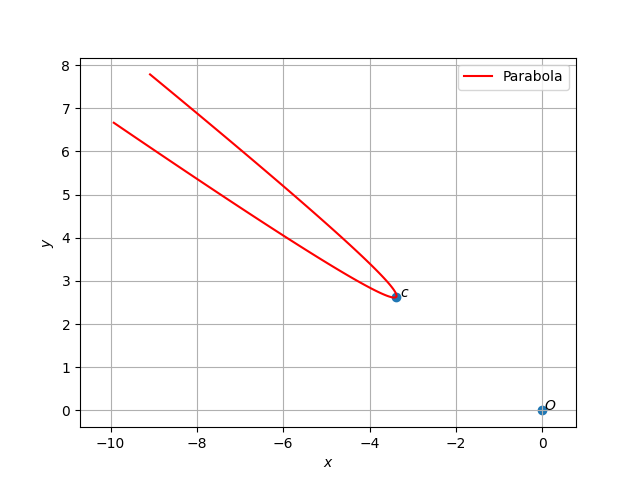
\includegraphics[width=\columnwidth]{parab.png}
        \caption{Graph of $9x^2+24xy+16y^2-4y-x+7=0$}
        \label{myfig}
\end{figure}
\end{document}
